\documentclass{article}
\usepackage{graphicx}
\graphicspath{ {images/} }

\title{The Book of Special Relativity}
\date{May 17th, 2017}
\author{Sishaar Rao}

\begin{document}
\pagenumbering{gobble}
\maketitle
\newpage
\pagenumbering{arabic}

Special relativity is a theory proposed by Albert Einstein that describes the propagation of matter and light at high speeds. It was invented to explain the observed behavior of electric and magnetic fields, which it beautifully reconciles into a single so-called electromagnetic field, and also to resolve a number of paradoxes that arise when considering travel at large speeds. Special relativity also explains the behavior of fast-traveling particle, including the fact that fast-traveling unstable particles appear to decay slower than identical particles traveling slower. Special relativity is an indispensable tool of modern physics, and its predictions have been experimentally tested time and time again without any discrepancies turning up. Special relativity reduces to Newtonian mechanics in the limit of small speeds.

\vspace{5mm}

According to special relativity, no wave or particle may travel at a speed greater than the speed of light c. Therefore, the usual rules from Newtonian mechanics do not apply when adding velocities that are large enough. For example, if a particle travels at a speed \( v \) with respect to a stationary observer, and another particle travels at a speed \( v' \)  with respect to the first particle, the speed \( u \) of particle two seen by the observer is not  as would be the case in Newtonian mechanics, but rather
\[
  u = \frac{v + v'}{1 + \frac{vv'}{c^2}}
\]

\newpage
\section{Invariance of Length’s Measured Perpendicular to Relative Motion}
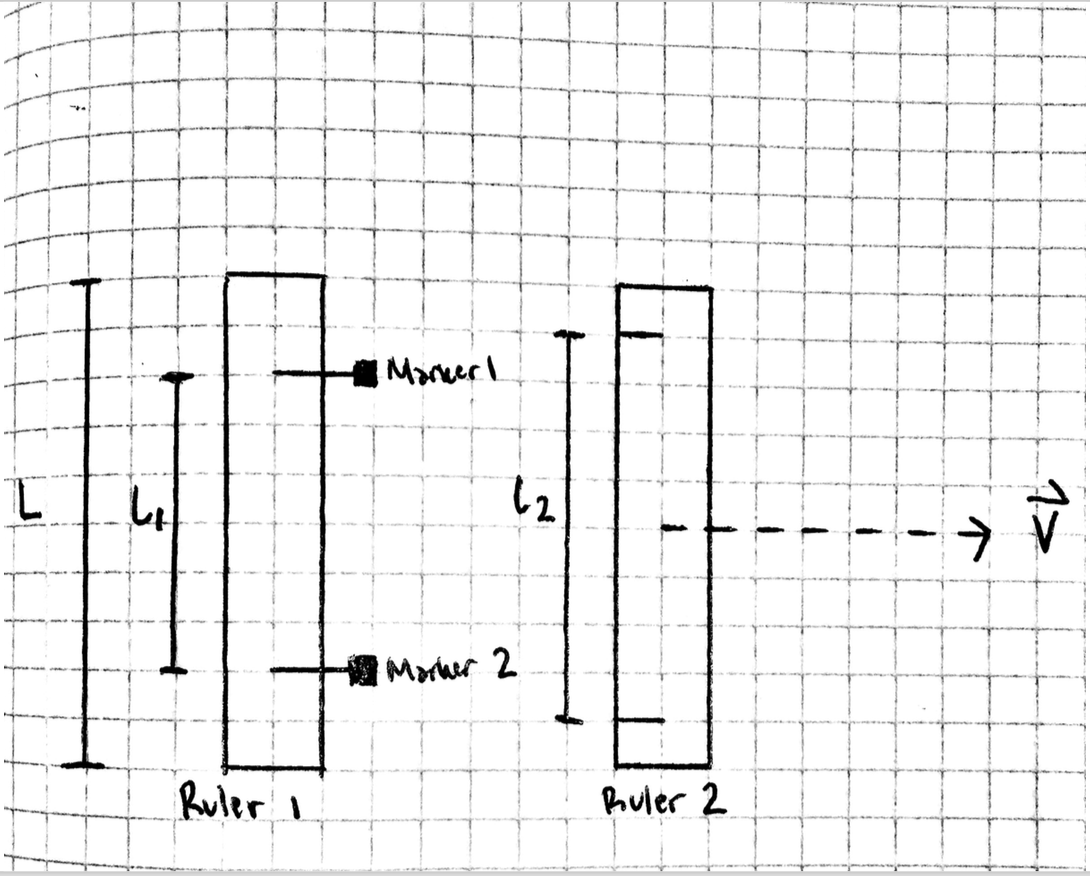
\includegraphics{sticks}
Figure 1.
  

\end{document}
